%-----------------------------------------------------------------------------%
\chapter{\babEmpat}
%-----------------------------------------------------------------------------%
Selama pelaksanaan Kerja Praktik di BMW Laboratory, NTUST, penulis terlibat dalam beberapa proyek utama dan kegiatan pendukung yang berfokus pada pengembangan ``Wifi RAN Digital Twin'' dan teknologi terkait. Bab ini akan merinci pelaksanaan kegiatan-kegiatan tersebut.

%-----------------------------------------------------------------------------%
\section{Masa Percobaan dan Pembelajaran Awal}
%-----------------------------------------------------------------------------%
Periode awal kerja praktik (4 April 2025 sampai 25 Juni 2025) difokuskan pada pembelajaran fundamental dan pengembangan kemampuan dasar yang menjadi landasan untuk proyek-proyek selanjutnya. Kegiatan pada masa ini dibagi menjadi tiga area utama: pemahaman alur kerja, penyiapan infrastruktur, dan pengembangan awal pengumpul data.
\subsection{Pemahaman Konsep dan Alur Kerja}
Tahap awal diisi dengan mempelajari alur kerja program magang TEEP, manajemen proyek menggunakan GitHub dan Trello, serta standar dokumentasi dengan Markdown. Penulis juga mempelajari konsep-konsep dasar yang relevan dengan proyek, termasuk arsitektur 5G, standar O-RAN, dan konsep Wifi.

\subsection{Pengembangan Awal Pengumpul Data}
Sebagai langkah awal untuk pengumpulan data, penulis meneliti berbagai metode untuk mengekstrak data dari perangkat jaringan Unifi. Metode \textit{web scraping} dipilih sebagai pendekatan awal. Penulis mempelajari pustaka Playwright dan berhasil mengembangkan skrip untuk secara otomatis masuk ke dasbor Unifi, menavigasi antarmuka, dan mengumpulkan data metrik dari \textit{Access Point} (AP). Skrip ini menjadi poin awal dari penulis mengembangkan \textit{WiFi Adapter} yang lebih kompleks di kemudian hari.

\begin{figure}[htbp]
    \centering
    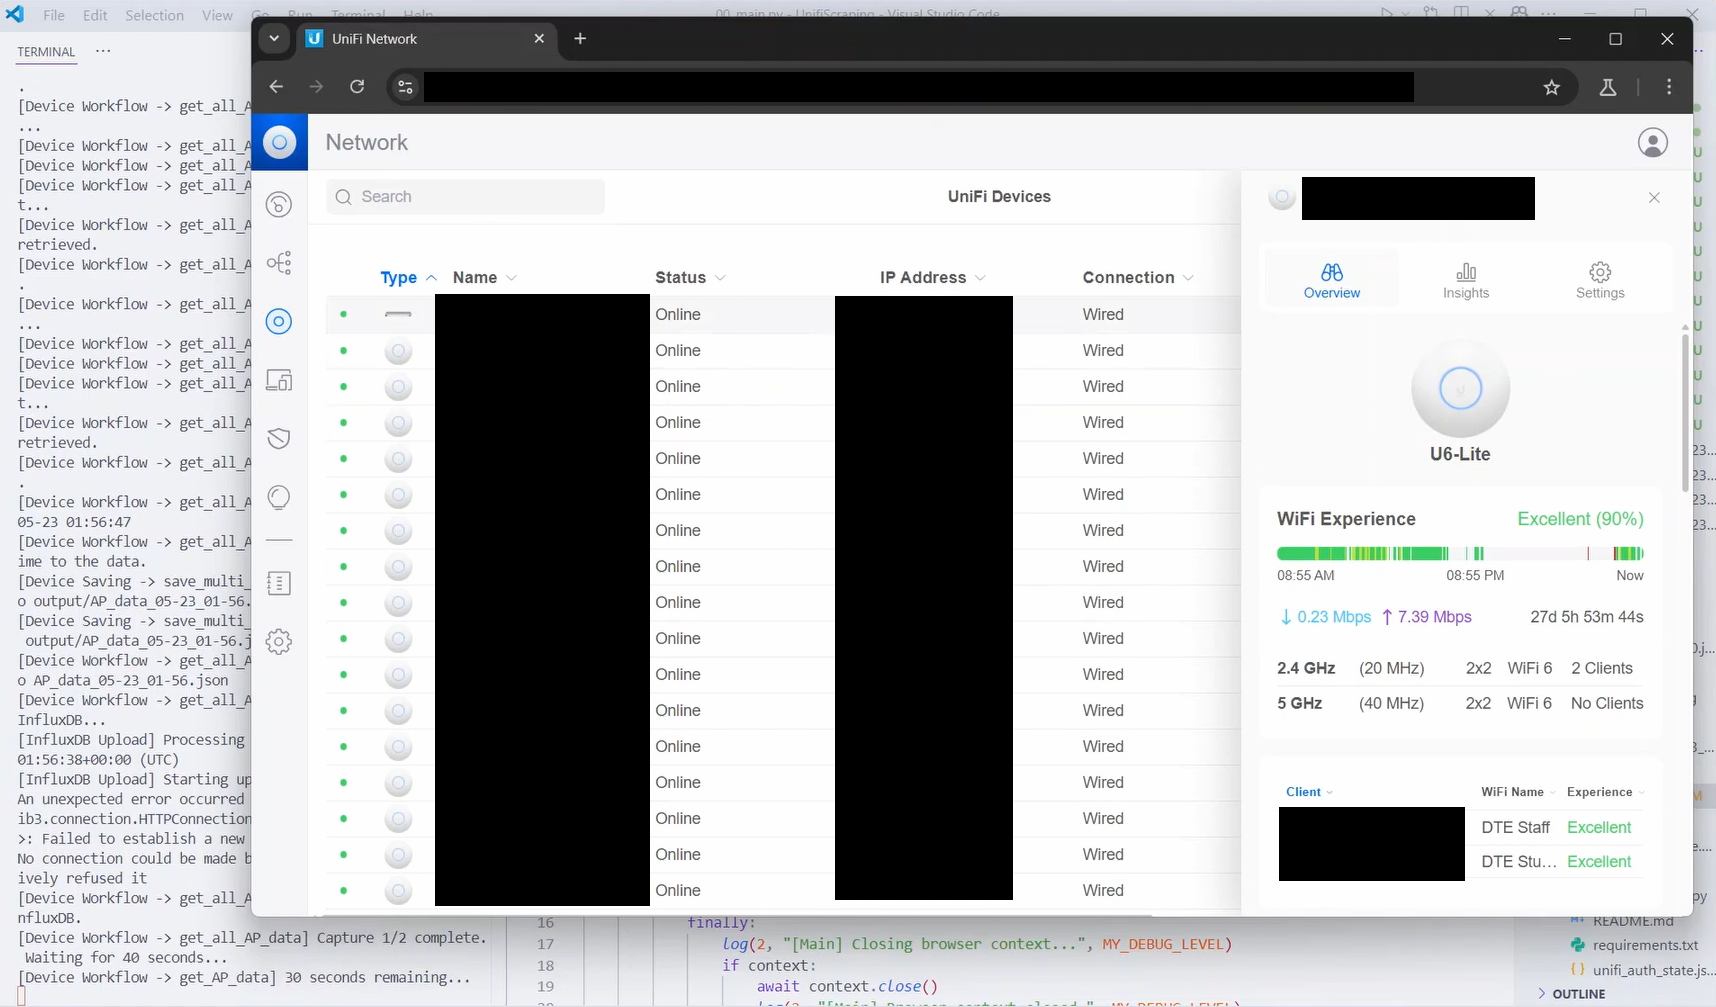
\includegraphics[width=0.8\textwidth]{assets/pics/unifi.png}
    \caption{Proses web scraping pada dasbor Ubiquiti Unifi, disensorkan untuk keamanan}
    \label{fig:unifi}
\end{figure}

Pengembangan skrip ini menggunakan struktur kode modular dan mengikuti format yang akan digunakan dalam \textit{WiFi Adapter} akhir. Dengan demikian, penulis dapat dengan mudah memahami alur kode WiFi Adapter yang dipakai di laboratorium.

Skrip menggunakan metode \textit{web scraping} dengan Playwright; saat program dijalankan, skrip akan membuka browser secara otomatis, masuk ke dasbor Unifi menggunakan kredensial yang disediakan, menavigasi ke halaman yang berisi metrik AP, dan mengekstrak data yang diperlukan untuk setiap AP (dapat dilihat pada Gambar \ref{fig:unifi}). Data yang dikumpulkan meliputi Nama AP, jumlah klien terhubung, dan statistik lalu lintas. Data ini kemudian diformat dan disimpan dalam file JSON (seperti yang ditunjukkan pada Gambar \ref{fig:unifijson}).

\begin{figure}[htbp]
    \centering
    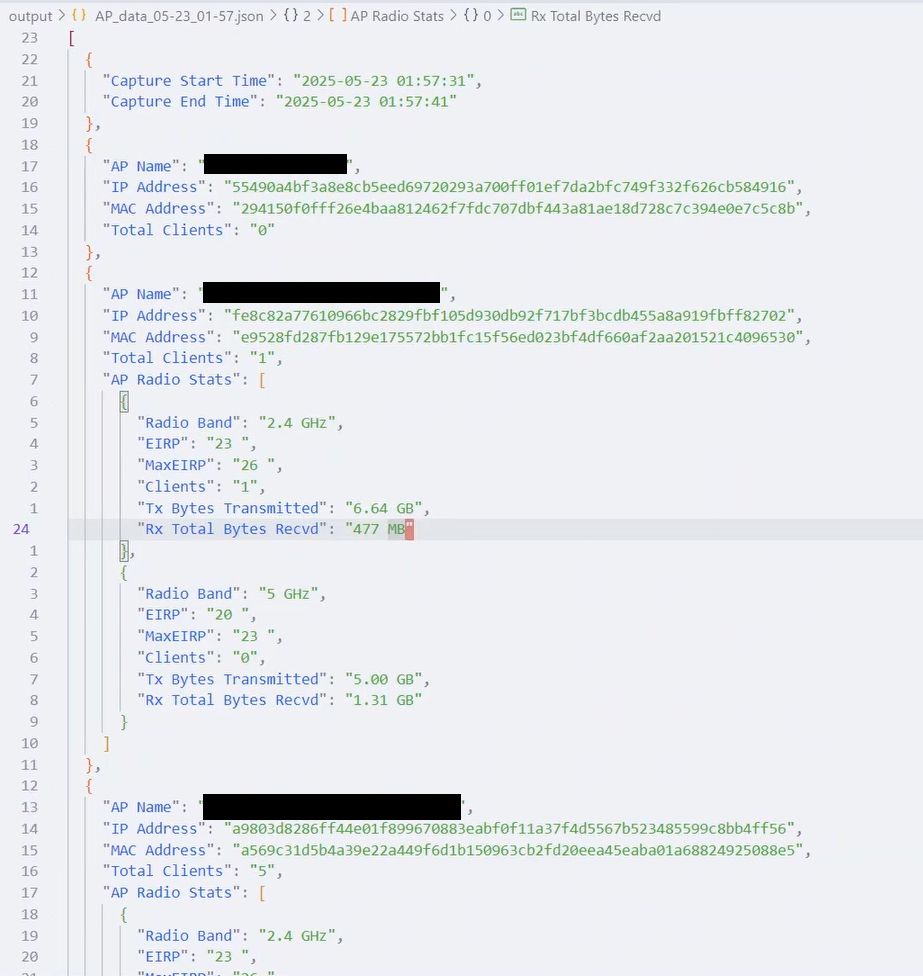
\includegraphics[width=0.5\textwidth]{assets/pics/unifijson.png}
    \caption{Data JSON yang dihasilkan dari proses web scraping, disensorkan untuk keamanan}
    \label{fig:unifijson}
\end{figure}


%-----------------------------------------------------------------------------%
\section{Proyek 1: WiFi Adapter untuk Integrasi O-RAN}
%-----------------------------------------------------------------------------%
Proyek ini bertujuan untuk membuat komponen perangkat lunak yang dapat mengumpulkan data dari infrastruktur WiFi di dunia nyata dan memformatnya agar sesuai dengan spesifikasi antarmuka O-RAN O1 untuk sistem \textit{Service Management and Orchestration} (SMO).

\subsection{Pengembangan dan Fungsionalitas}
Tahap awal pengembangan berfokus pada implementasi \textit{WiFi Adapter} untuk mengirimkan data \textit{Performance Management} (PM) ke SMO. Data ini mencakup metrik penting seperti RSSI dan jumlah klien, yang diformat sebagai laporan berbasis file (JSON/XML) dan dikirim melalui SFTP.

Untuk mendukung interoperabilitas, arsitektur adapter dirancang secara modular dengan beberapa kelas utama: \textit{Connection, Crawler, Converter, Vault,} dan \textit{Database}. Fokus utama adalah pada implementasi untuk perangkat dari vendor Aruba dan HPE. Skrip Python dikembangkan untuk mengekstrak metadata dari \textit{Access Point} (AP) Aruba dan switch HPE menggunakan protokol SNMP.
\begin{itemize}
    \item \textbf{Data AP Aruba yang Dikumpulkan:} Nama host AP (\textit{AP\_Name}), alamat IP manajemen, alamat MAC, model AP (\textit{AP Type}), pita frekuensi radio (\textit{radio\_band}), dan detail SSID/BSSID.
    \item \textbf{Data Switch HPE yang Dikumpulkan:} Data pemetaan port yang menghubungkan perangkat (AP) ke port switch fisik, termasuk \textit{Port Name}, \textit{Switch Hostname}, dan \textit{PoE Type}.
\end{itemize}
Selama pengembangan, penulis melakukan pengujian \textit{crawling} PoE, debugging masalah \textit{crawling} RSSI, menangani pengambilan kredensial dari beberapa database, dan mencocokkan parameter agar sesuai dengan standar O-RAN.

\subsection{Integrasi dengan SMO}
Tahap selanjutnya adalah mengintegrasikan data yang dikumpulkan dengan struktur PM di SMO. Kegiatan pada tahap ini meliputi:
\begin{itemize}
    \item Memperbaiki kesalahan pada format XML PM agar sesuai dengan ekspektasi SMO.
    \item Mengedit label dan melakukan sanitasi data.
    \item Mengimplementasikan fitur seperti penghapusan file PM dan pengaturan tanggal kedaluwarsa file.
    \item Mempersiapkan integrasi NETCONF dengan menginstal pustaka yang diperlukan di lingkungan server.
\end{itemize}
Kegiatan integrasi SMO ini sebagian besar dilakukan pada awal Oktober 2025.

%-----------------------------------------------------------------------------%
\section{Proyek 2: Simulator RSSI Sionna dan Pipeline Lokalisasi}
%-----------------------------------------------------------------------------%
Proyek ini merupakan inti dari penelitian ``Wifi RAN Digital Twin'', yang berfokus pada pembuatan lingkungan kembaran digital untuk analisis propagasi sinyal dan pemodelan lokalisasi.

\subsection{Pengembangan Aplikasi Simulator Sionna}
Penulis mengembangkan aplikasi Python bernama \texttt{RSSI\_App.py} yang menggunakan NVIDIA Sionna untuk menyimulasikan propagasi sinyal dan memperkirakan nilai RSSI. Arsitektur aplikasi, diagram kelas, dan diagram urutan juga dirancang untuk mendokumentasikan sistem. Untuk simulasi, sebuah lingkungan 3D dari denah lantai gedung dibuat menggunakan Blender.

Salah satu bagian penting dari proyek ini adalah kalibrasi parameter. Metode \textit{parameter sweeping} diimplementasikan untuk mengeksplorasi efek dari berbagai parameter, seperti efek material (konduktivitas, permitivitas, koefisien hamburan, dan ketebalan dinding). Metode optimisasi hibrida yang menggabungkan CMA-ES dan Adam (\texttt{06\_hybrid-optimization\_4-params.py}) digunakan untuk menyetel parameter simulasi agar hasilnya cocok dengan data RSSI yang diukur di dunia nyata. Aplikasi ini menghasilkan output berupa \textit{heatmap}, plot, dan dataset sidik jari.

\subsection{Implementasi Pipeline Lokalisasi}
Sebagai bukti konsep (\textit{Proof-of-Concept}), model lokalisasi sederhana dikembangkan menggunakan K-Nearest Neighbors (KNN) dan dataset sederhana. Selain itu, model klasifikasi ruangan juga dibuat.

Pipeline lokalisasi yang lebih lengkap diimplementasikan dengan alur sebagai berikut:
\begin{enumerate}
    \item Dataset sidik jari dihasilkan menggunakan parameter simulasi yang telah dikalibrasi.
    \item Eksperimen lokalisasi KNN dijalankan (\texttt{02\_rssi-knn-for-ap.ipynb}) menggunakan sidik jari yang dihasilkan dan dibandingkan dengan data RSSI AP dari dunia nyata.
    \item Selain itu, penulis juga menjalankan kembali dan memodifikasi eksperimen lokalisasi \textit{Rogue AP} berbasis XGBoost yang sudah ada sebelumnya, dan mengintegrasikan Sionna untuk visualisasi/pemetaan lokasi yang diprediksi.
\end{enumerate}

%-----------------------------------------------------------------------------%
\section{Proyek 3: Layanan Sinkronisasi GitHub ke Trello}
%-----------------------------------------------------------------------------%
Penulis memberikan kontribusi signifikan dalam meningkatkan dan memelihara layanan sinkronisasi dua arah yang dirancang untuk menyelaraskan log harian dan \textit{milestone} antara file Markdown di GitHub dan kartu di Trello.

Pekerjaan berpusat pada debugging, finalisasi, dan refaktorisasi basis kode. Beberapa perbaikan bug kritis yang berhasil diselesaikan antara lain:
\begin{itemize}
    \item \textbf{Efek ``Ping-Pong'':} Masalah yang disebabkan oleh perbedaan stempel waktu kecil yang menyebabkan sinkronisasi berulang tanpa henti.
    \item \textbf{Batas 50 Komentar API Trello:} Diatasi dengan mengimplementasikan paginasi berbasis kursor.
    \item \textbf{Duplikasi Aturan Horizontal:} Memperbaiki kesalahan pemformatan Markdown.
\end{itemize}
Selain perbaikan bug, fitur baru juga dikembangkan, yaitu resolusi konflik antar komentar yang dapat dikonfigurasi. Fitur ini memungkinkan pengguna memilih strategi resolusi, seperti \texttt{more\_recent} (berdasarkan stempel waktu) atau \texttt{more\_characters} (mempertahankan konten yang lebih detail). Penulis juga membuat dokumentasi yang komprehensif (termasuk dokumentasi Sphinx) dan video demo untuk alat ini.

%-----------------------------------------------------------------------------%
\section{Riset, Analisis, dan Aktivitas Pendukung}
%-----------------------------------------------------------------------------%
Selain proyek-proyek utama, penulis juga terlibat dalam berbagai kegiatan penelitian, analisis, dan pendukung.

\subsection{Pengumpulan Data Awal dengan Web Scraping}

Sebelum implementasi \textit{WiFi Adapter} berbasis SNMP, fokus awal adalah mengumpulkan data dari perangkat Ubiquiti Unifi menggunakan \textit{web scraping}. Penulis meneliti berbagai metode pengumpulan data dan memilih Playwright untuk melakukan \textit{scraping} pada dasbor Unifi. Skrip yang dikembangkan mampu menangani login, navigasi, menangkap data AP secara berkala (Nama AP, Alamat IP, Klien, Throughput, dll.), melakukan hashing pada alamat IP/MAC, dan menyimpan data ke format JSON atau mengunggahnya langsung ke InfluxDB.


\subsection{Studi Konsep O-RAN dan Wifi RAN}
Penulis mempelajari standar O-RAN, dengan fokus pada Spesifikasi Antarmuka O1 (WG10). Dari studi ini, tiga fase untuk pengembangan \textit{WiFi Adapter} diformalkan: 1) pengiriman data PM melalui VES/SFTP, 2) konfigurasi melalui NETCONF, dan 3) kontrol penuh SMO sebagai produsen MNS.

\subsection{Analisis Kasus Penggunaan Data WiFi}
Penulis menganalisis berbagai kasus penggunaan data WiFi, termasuk prediksi beban untuk penghematan energi, estimasi propagasi AP menggunakan Sionna, pembuatan profil pergerakan pengguna, deteksi anomali tanpa pengawasan, dan analisis waktu tinggal (\textit{dwell-time}). Analisis data RSSI juga dilakukan, di mana penulis mempelajari konsep dasar elektromagnetik dan analisis deret waktu.

\subsection{Logistik dan Dokumentasi}
Tugas-tugas lain yang dilakukan meliputi:
\begin{itemize}
    \item \textbf{Administrasi/Infrastruktur:} Memperbaiki masalah pada server/PC lab (akses Proxmox, masalah login Ubuntu, mengambil perangkat keras lab, dan menangani penyimpanan penuh pada server InfluxDB).
    \item \textbf{Pengembangan Situs Web Lab:} Mengerjakan perombakan komprehensif situs web BMW Lab menggunakan Google Sites.
    \item \textbf{Dokumentasi Resmi:} Menyusun log KP dan laporan KP menggunakan LaTeX, membuat dan merevisi video testimoni dan penjelasan proyek, serta menyiapkan berbagai slide presentasi.
    \item \textbf{Manajemen Peserta Magang Baru:} Membuat sumber daya pembelajaran, rencana studi, dan tugas untuk peserta magang baru.
\end{itemize}